\documentclass[12pt,a4paper]{article}

\usepackage[utf8]{inputenc}
\usepackage[T1]{fontenc}
\usepackage[spanish]{babel}
\usepackage{graphicx}
\usepackage{float}

\begin{document}
	
	\section{Prototipo de Interfaces}
	
	Con el objetivo de validar la experiencia de usuario y visualizar el alcance funcional de la plataforma, se desarrolló un prototipo de interfaces que representa las principales pantallas del sistema. Estas interfaces permiten identificar los módulos disponibles para cada tipo de usuario y facilitan la evaluación temprana de la usabilidad de la solución propuesta.
	
	Las siguientes figuras muestran las pantallas diseñadas para los diferentes actores del sistema.
	
	\subsection{Página de Inicio}
	
	La página de inicio constituye el punto de acceso principal a la plataforma. En ella se presentan los objetivos generales del sistema, los beneficios para comercializadoras y vendedores, así como las opciones de autenticación y registro.
	
	\begin{figure}[H]
		\centering
		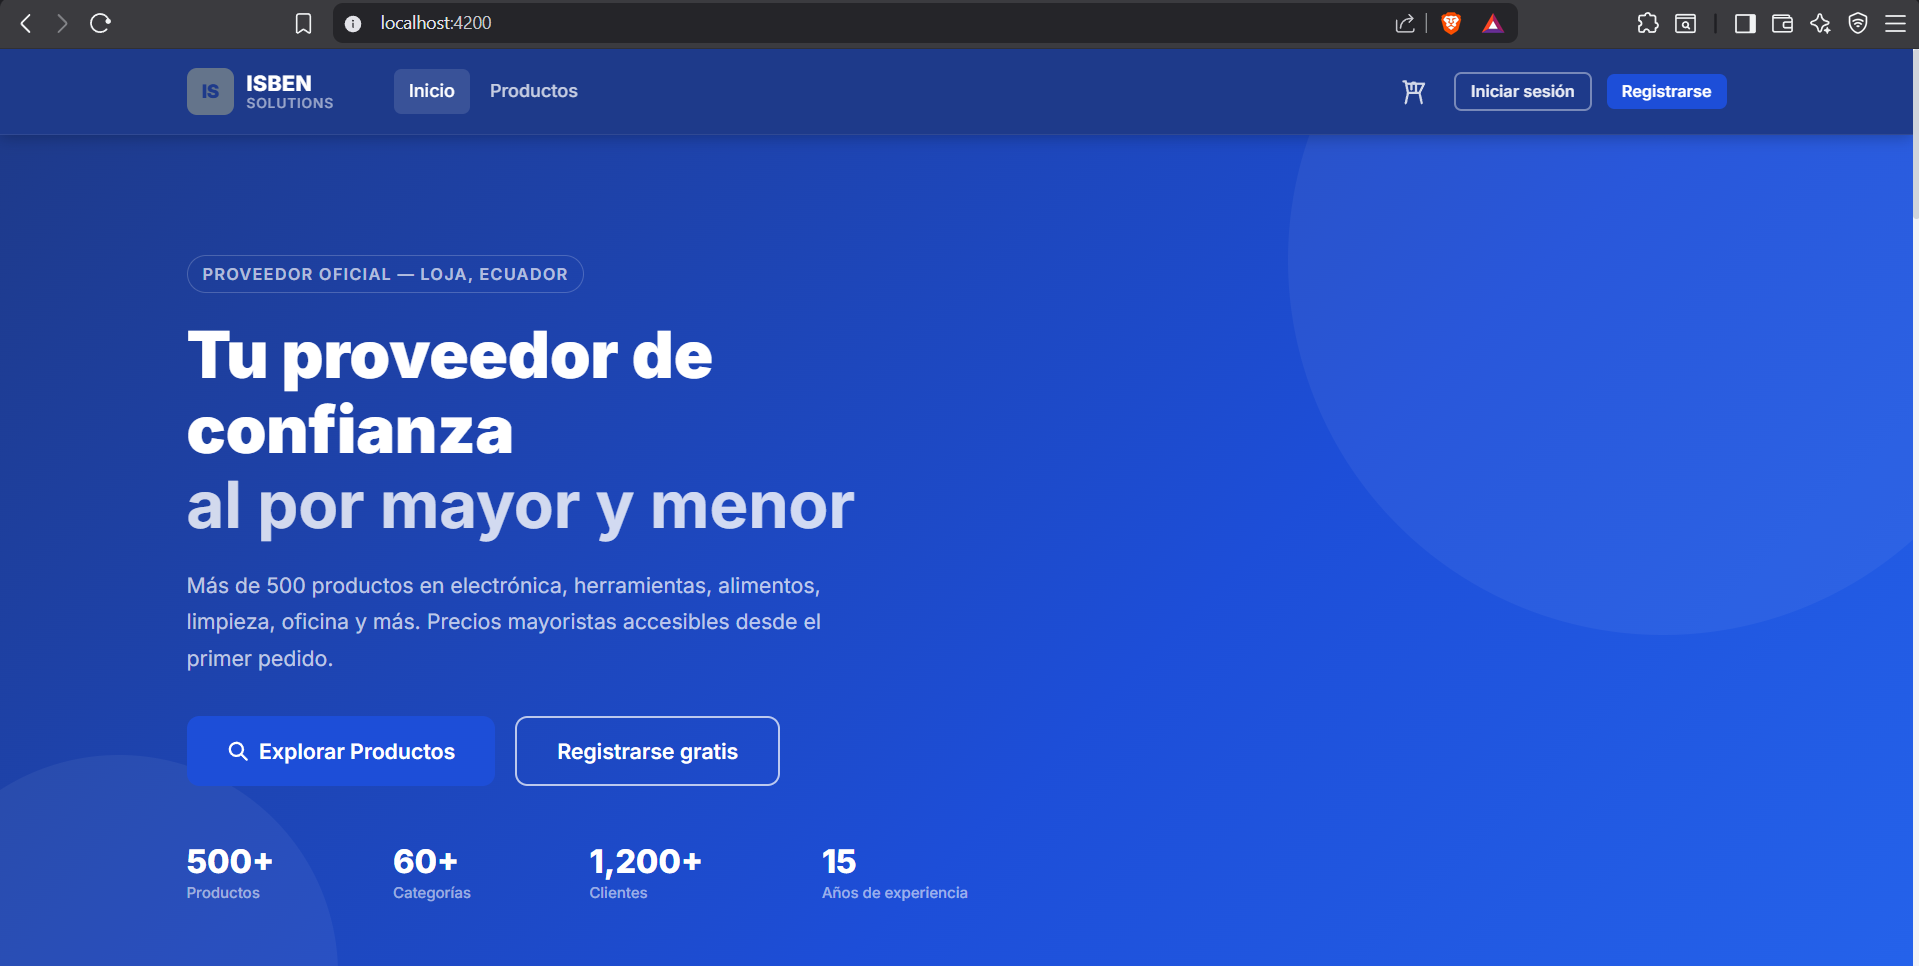
\includegraphics[width=0.9\textwidth]{imagenes/index.png}
		\caption{Página principal de la plataforma}
		\label{fig:inicio}
	\end{figure}
	
	\subsection{Inicio de Sesión}
	
	La interfaz de autenticación permite a los usuarios acceder a las funcionalidades correspondientes a su rol dentro de la plataforma.
	
	\begin{figure}[H]
		\centering
		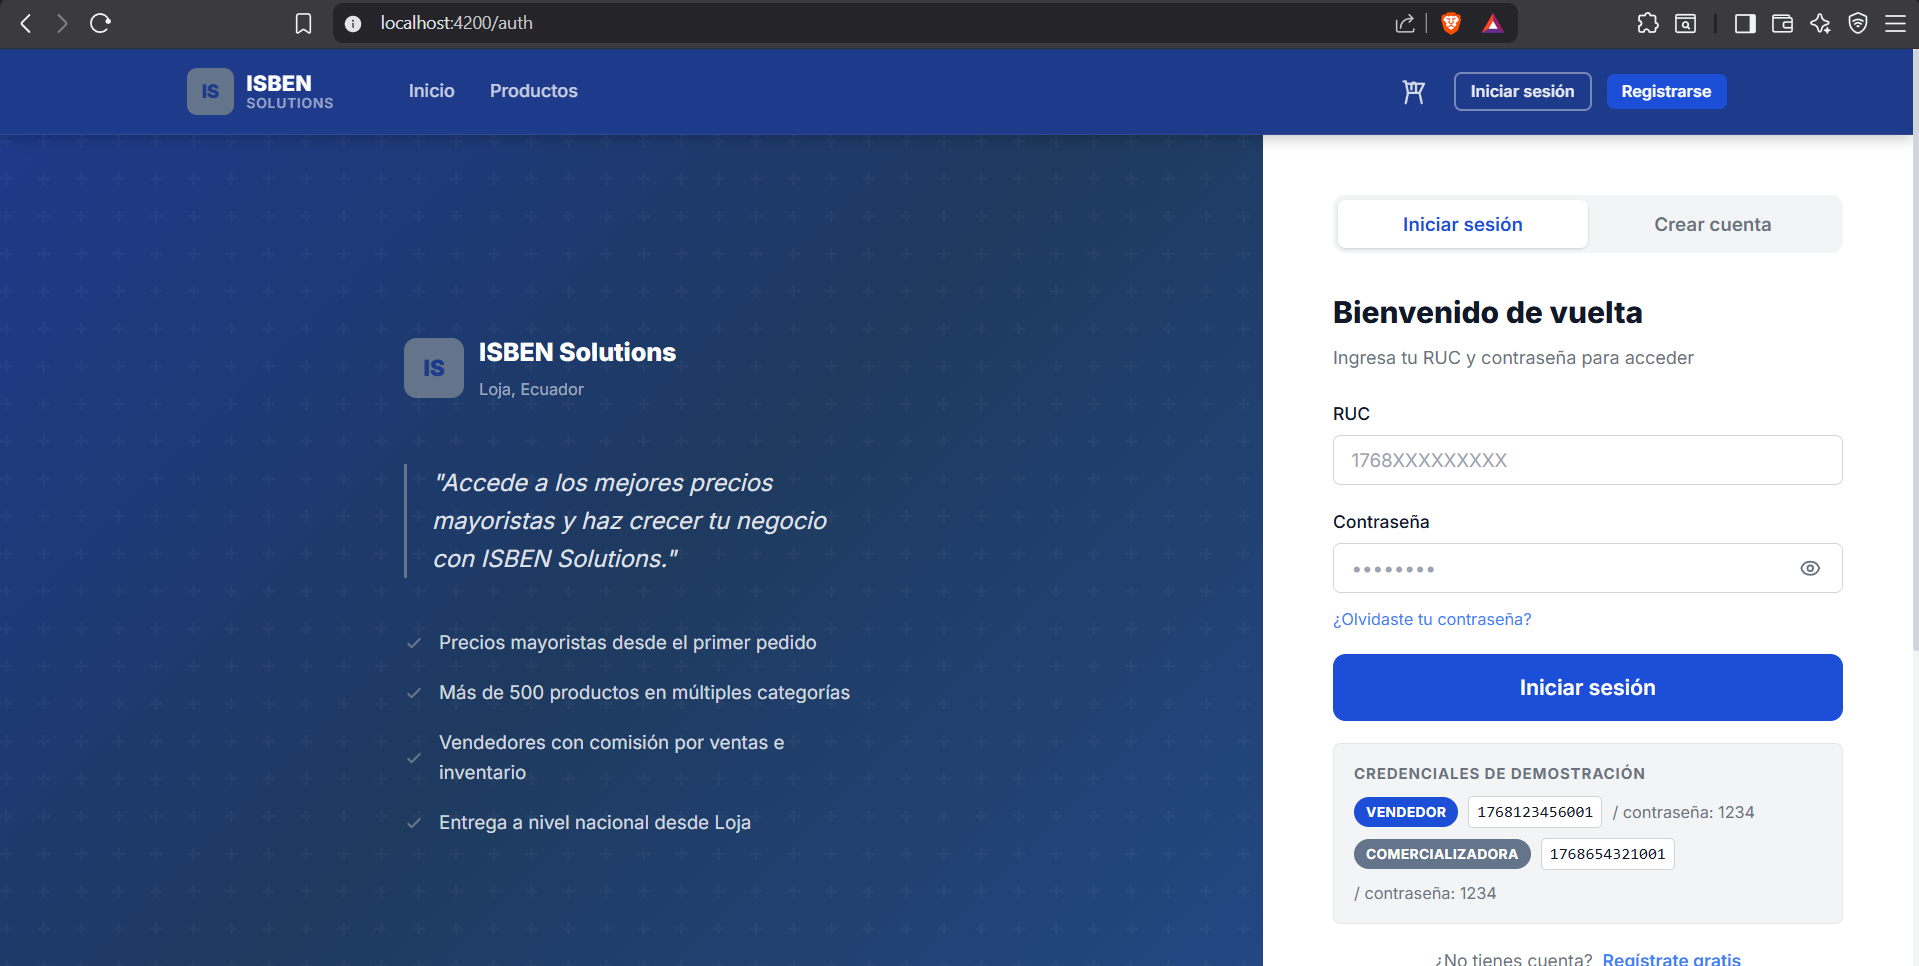
\includegraphics[width=0.8\textwidth]{imagenes/inicio_sesion.png}
		\caption{Pantalla de inicio de sesión}
		\label{fig:login}
	\end{figure}
	
	\subsection{Registro de Usuarios}
	
	Esta interfaz permite registrar nuevos usuarios dentro del sistema, diferenciando entre comercializadoras y vendedores independientes.
	
	\begin{figure}[H]
		\centering
		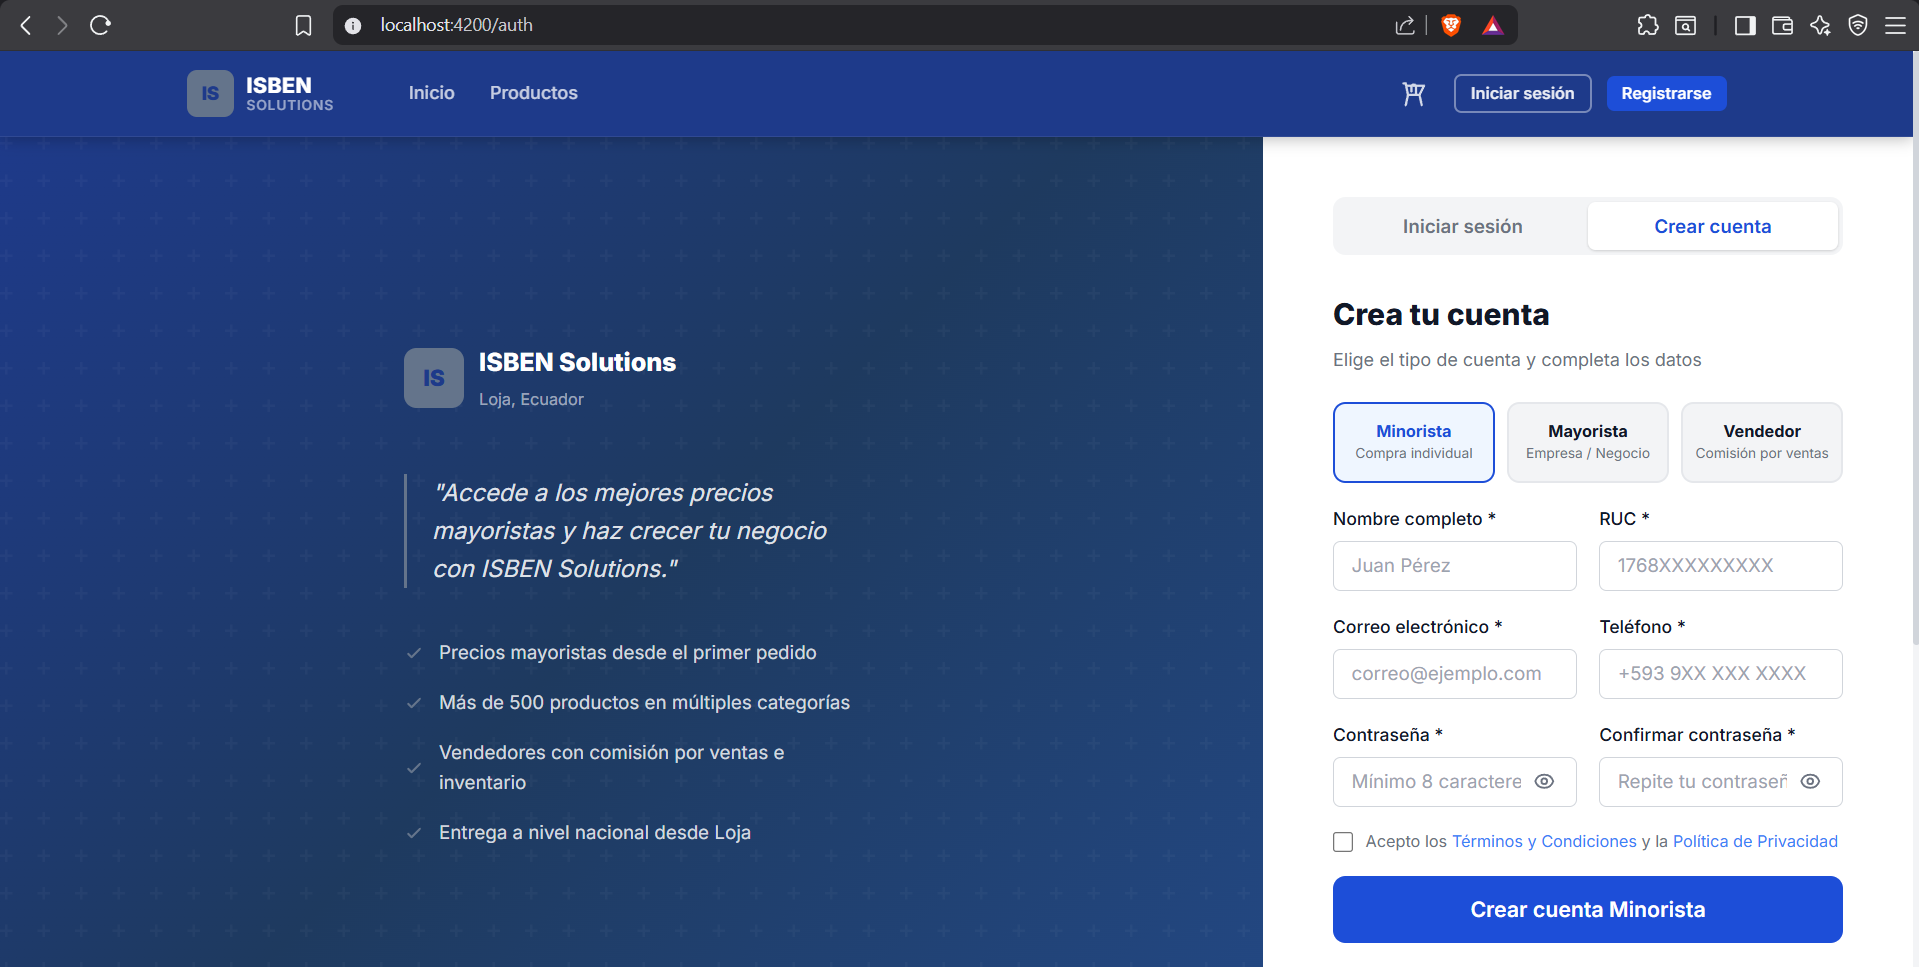
\includegraphics[width=0.8\textwidth]{imagenes/registro.png}
		\caption{Pantalla de registro}
		\label{fig:registro}
	\end{figure}
	
	\subsection{Dashboard de Comercializadora}
	
	El panel de comercializadora proporciona acceso a la gestión de productos, inventario, pedidos y reportes operativos.
	
	\begin{figure}[H]
		\centering
		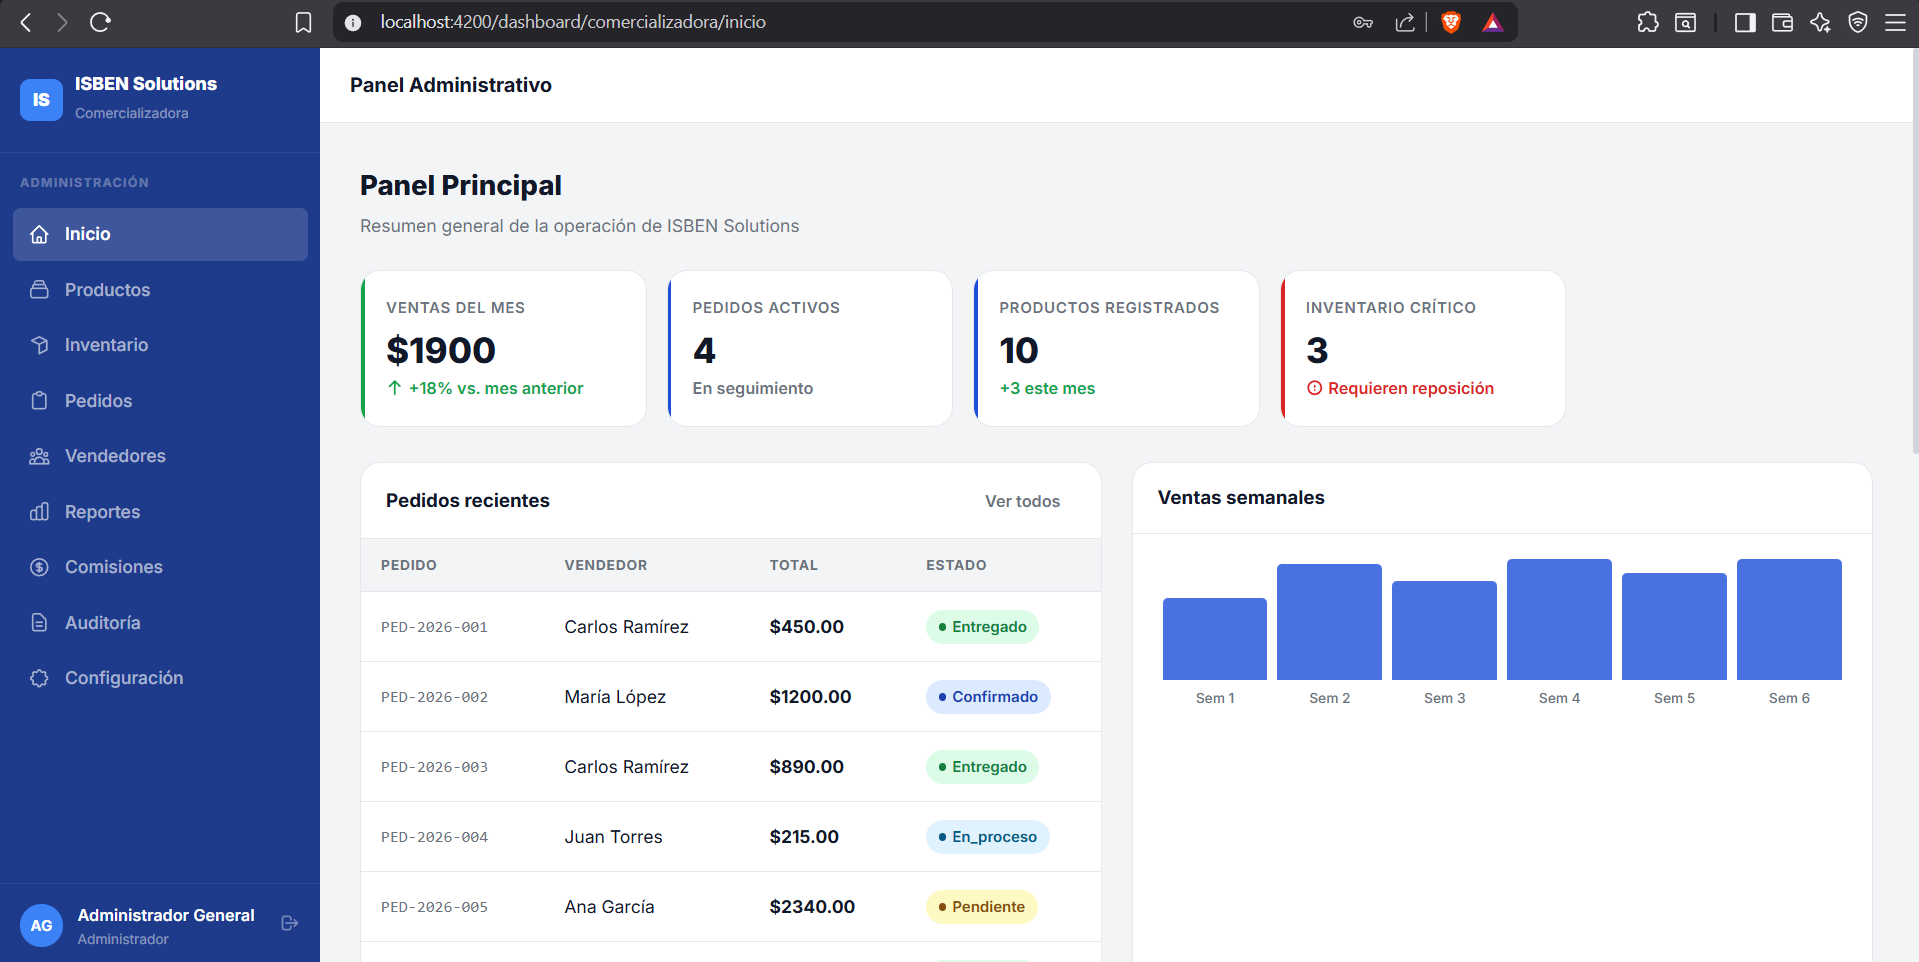
\includegraphics[width=0.95\textwidth]{imagenes/panel_comercializadora.png}
		\caption{Dashboard de comercializadora}
		\label{fig:dashboard_comercializadora}
	\end{figure}
	
	\subsection{Dashboard de Vendedor}
	
	El panel de vendedor permite consultar productos, registrar pedidos, visualizar comisiones y gestionar recompensas.
	
	\begin{figure}[H]
		\centering
		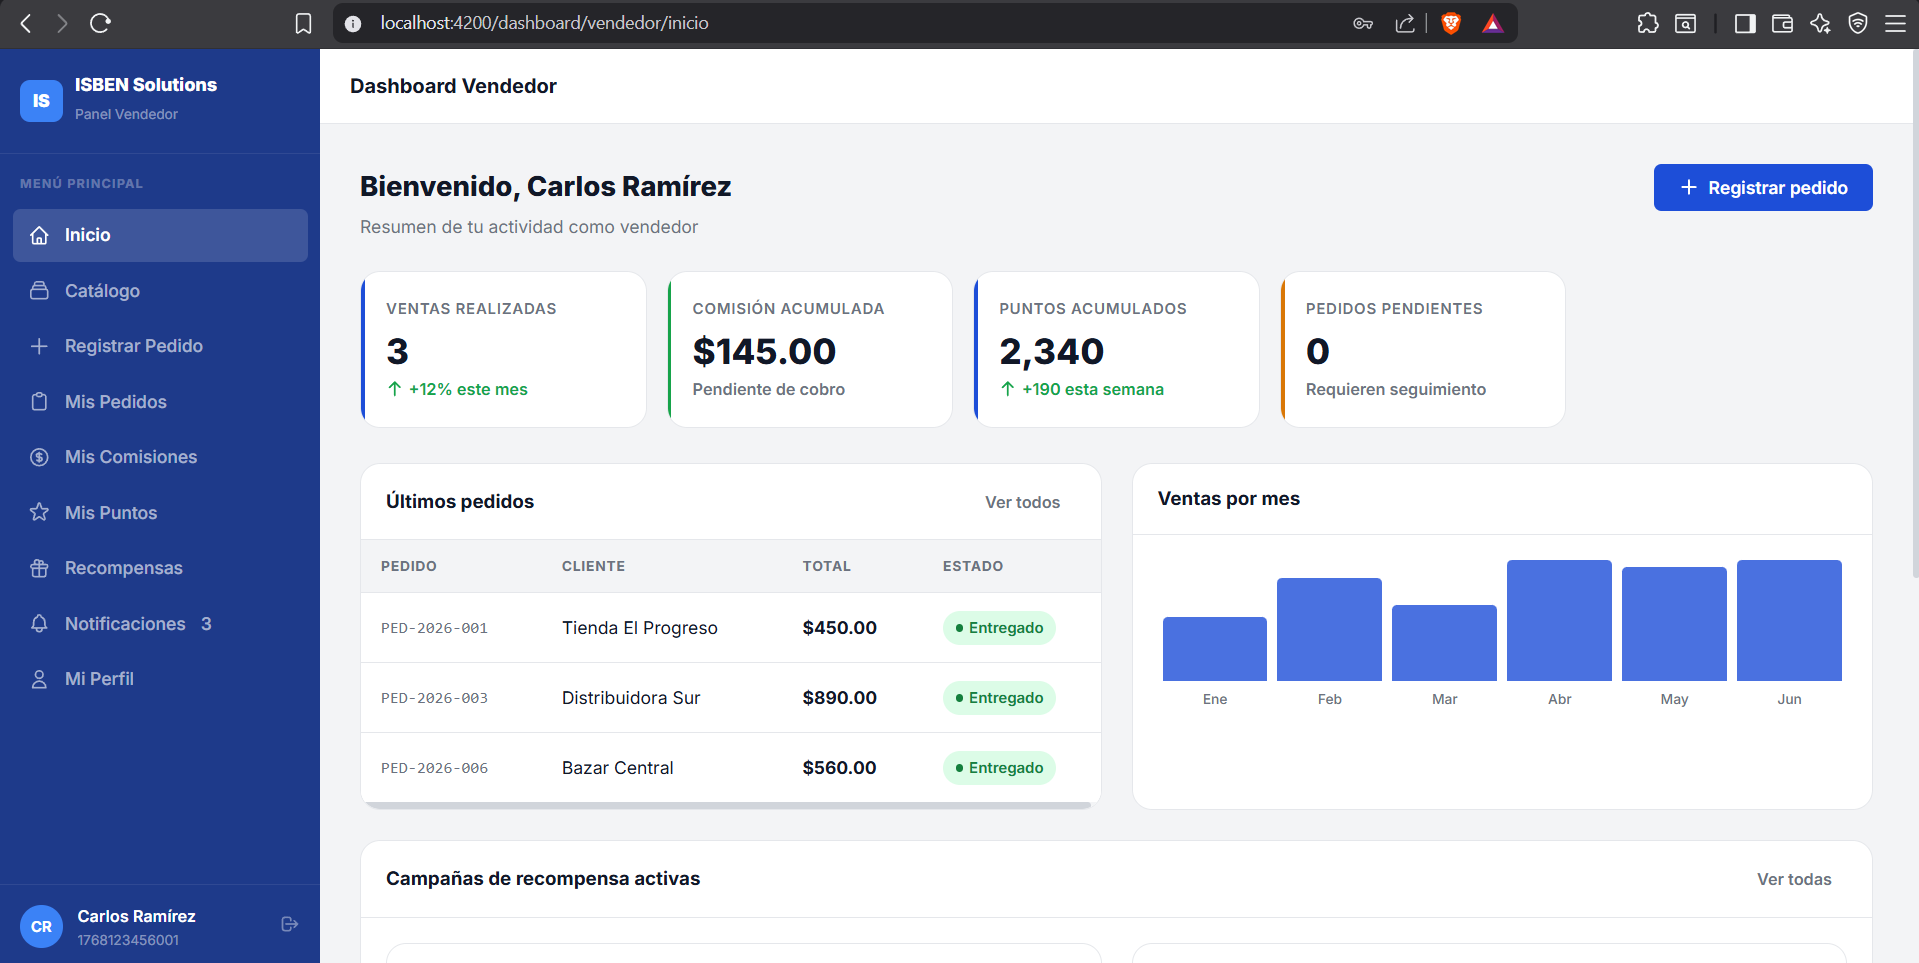
\includegraphics[width=0.95\textwidth]{imagenes/panel_vendedor.png}
		\caption{Dashboard de vendedor}
		\label{fig:dashboard_vendedor}
	\end{figure}
	
	\subsection{Dashboard de Administración}
	
	La interfaz administrativa permite supervisar el funcionamiento general de la plataforma, gestionar usuarios y acceder a reportes estratégicos.
	
	\begin{figure}[H]
		\centering
		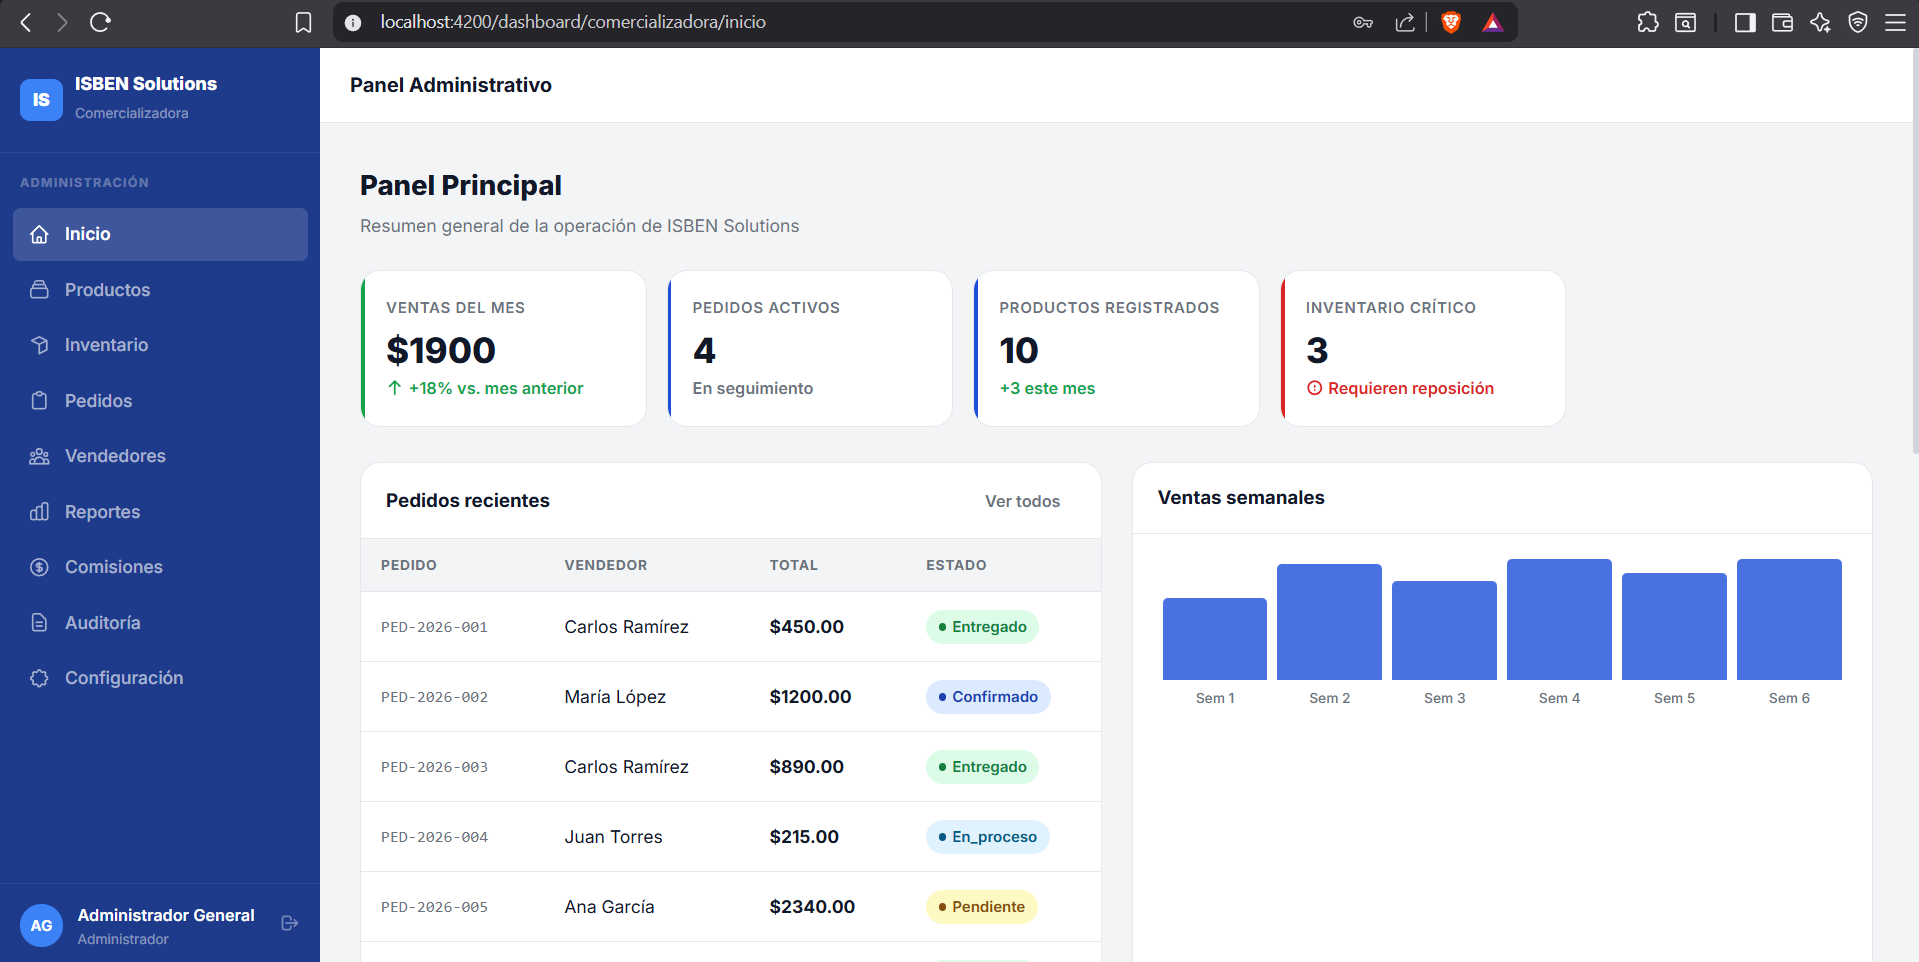
\includegraphics[width=0.95\textwidth]{imagenes/panel_comercializadora.png}
		\caption{Dashboard de administración}
		\label{fig:dashboard_administrador}
	\end{figure}
	
	Es importante señalar que las interfaces presentadas en esta sección corresponden únicamente a las pantallas principales del prototipo, seleccionadas con el fin de ilustrar los flujos más representativos del sistema y las funcionalidades esenciales de cada tipo de usuario. Sin embargo, el proyecto contempla interfaces adicionales relacionadas con la gestión de productos, inventario, pedidos, comisiones, reportes, auditorías y configuraciones específicas de cada rol. Dichas interfaces forman parte de la implementación desarrollada y pueden consultarse en el código fuente disponible dentro de la carpeta \texttt{interfaz}, donde se encuentran los componentes y vistas complementarias que amplían el alcance funcional de la plataforma.
	
\end{document}